\chapter{Grundlagen} 
\label{ch:grundlagen}
In diesem Kapitel möchte ich einige Grundlagen für die weiteren Kapitel dieser Arbeit legen. Zunächst erläutere ich den Aufbau eines neuronalen Netzes im allgemeinen, die Bedeutung von rekurrenten neuronalen Netzen (RNN), zeige am Bouncing Ball Szenario das Vanishing Gradient Problem auf und mache so die Notwendigkeit der LSTM-Technik deutlich.
\section{Neuronale Netze}

\begin{figure}
	\centering
	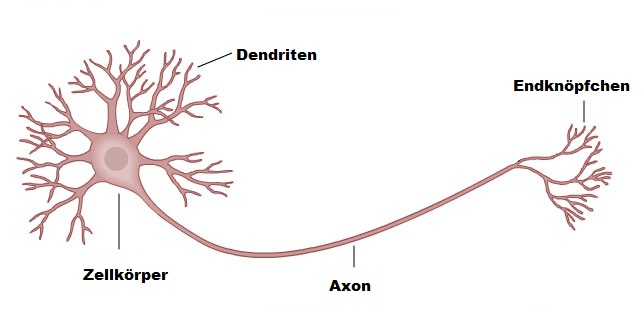
\includegraphics[width=0.7\textwidth, height=150px]{pics/neuron.jpg}	
	\caption{Schematische Darstellung eines biologischen Neuron \cite{bib:neuron}}
	
	\label{img:neuron}
\end{figure}
\begin{figure}
	\centering
	
	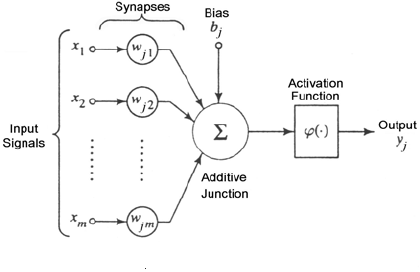
\includegraphics[width=0.7\textwidth, height=150px]{pics/aneuron.png}	
	\caption{Schematische Darstellung eines künstlichen Neuron \cite{bib:aneuron}}
	\label{img:aneuron}
\end{figure}

Als neuronales Netz bezeichnet man eine verwobene Struktur zwischen vielen einzelnen Zellen von meistens gleichem - aber keineswegs darauf beschr\"anktem - Aufbau, den sogenannten Neuronen. Eine solche Zelle hat immer die Eigenschaft, dass sie Signale von anderen Zellen empfängt, diese gewichtet aufakkumuliert und abhängig von einer internen Aktivierungsfunktion ein entsprechendes Signal an andere Zellen weitergibt, die damit ihrerseits diesselbe Prozedur durchlaufen. Ein neuronales Netz im Gehirn einer Ameise hat ca. 250.000 Neuronen, ein menschliches 86 Milliarden (1) und wir haben lediglich eine wage Vorstellung, wozu diese imstande sind. In der Informatik werden solche Strukturen als künstliche neuronale Netze nachgebildet und je nach Problemstellung abgewandelt. Zur Vereinfachung meinen wir ab sofort, sofern nicht explizit anders angegeben, mit neuronalen Netzen künstliche neuronale Netze.
\begin{figure}
	\centering
	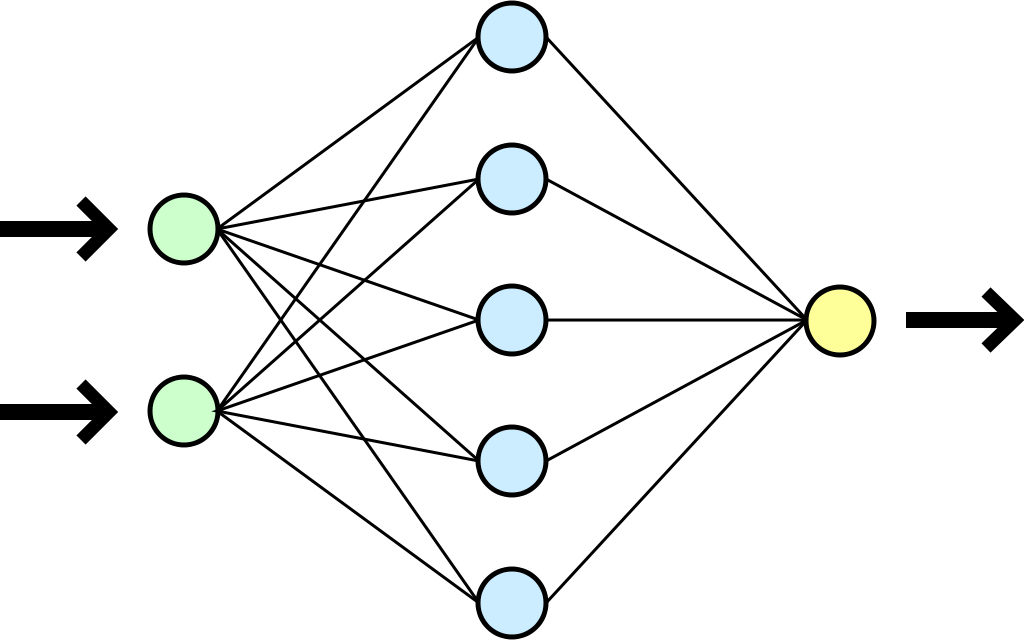
\includegraphics[width=0.7\textwidth, height=150px]{pics/MLP.png}	
	\caption{Ein Multilayer Perceptron mit 2 Inputneuronen(grün), einem Hidden Layer mit 5 Neuronen(blau) und einem einzelnen Outputneuron(gelb).   \cite{bib:mlp}}
	\label{img:aneuron}
\end{figure}
Es gibt viele verschiedene Arten von neuronalen Netzen, die einfachste von Ihnen ist das Multilayer Perceptron (MLP). Die Zellen werden zu mehreren Ebenen(Layer) zusammengefügt und es gibt eine geordnete Datenflussrichtung, eine Zelle erhält ihren Input von jeder Zelle der vorigenen Ebene und gibt ihren Output entsprechend an jede Zelle der folgenden Ebene weiter, Feedforward genannt (Vgl Bild 2). 
Bild 3 Künstliches Neuron 
Gl 1: xh = phi,h(net(h)) = phi,h(Sigma i€I (wih xi))
In jeder Zelle werden die Inputsignale, also die Aktivierungen der vorigen Zellen aufsummiert, aber unterschiedlich gewichtet vgl GL 1. Eben diese Gewichte sind der Kern des maschinellen Lernens, da bei einmal geschickt gefundenen Gewichten, komplexe Aufgabenstellungen und Probleme mit (vergleichsweise) wenig Rechen- sowie Programmieraufwand gelößt werden können. Im Wesentlichen versucht ein MLP immer eine Funktion zu berechnen welches einen Inputvektor der Größe n auf einen Outputvektor der Größe m abbildet. 
FM: R^n -> R^m (2 Seite 11). 
Ein Beispiel für eine solche Funktion wäre für ein gegebenes Bild zu entscheiden, ob darauf ein Gesicht zu erkennen ist. Die Länge des Inputs wäre hier z.B. mehrere Millionen, einfach die Pixelwerte, als Output wäre hier nur eine Zahl, nämlich ob ein Gesicht zu sehen ist oder nicht. Der Output y des Netzes ist also abhängig vom Input x, aber auch von den Gewichten w.
Die Gewichte werden entweder mit Hilfe von Trainingsdaten, bestehend aus Inputdaten und entsprechenden Outputdaten, also den zugehören Lösungen, oder mit einer zu erlenenden Zielfunktion, die einem aus gegebenen Inputdaten die gewünschten Lösungen liefert, über mehrere Trainingsläufe (Epochen) justiert. Fügt man in das Input-Layer entsprechende Inputdaten x ein, berechnet die Aktivierungen aller Zellen, vergleicht die Aktivierungen y des Outputlayers des Netzes mit den gegebenen Lösungen z und erhält eine Fehlerabweichung E(z,y) (GL2). 
Gl 2: E(z,y) =def 1/2 Sigma.i=1.m (zi-yi)²
Die Herausforderung ist es nun, diejenigen Gewichte w zu finden, für die die Fehlerabweichung über alle Trainingsdaten minimal ist.
GL 3: arg min w sigma(x,z)€trainset E(z,fM(w,x)).
Geläufig ist hier der Backpropagation-Algorithmus. 
Code einfügen? 
\section{Rekurrente Neuronale Netze}

Neuronale Netzwerke haben einen für einen 1-Dimensionalen Input einen klar definierten 1-Dimensionalen Output und für die meisten Problemstellungen ist auch genau diese Kompetenz gefordert. Es gibt aber auch Probleme, bei denen der Output nicht nur von diesem, sondern auch von allen beziehungsweise einigen vorigen Inputs / Zuständen abhängt. Ein anschauliches Beispiel wäre hier die Klassifizierung von Videoausschnitten, wo die Bedeutung eines einzelnen Frames vom Kontext der vorigen Frames abhängt, hingegen ein einfacheres Beispiel wäre das in dieser Arbeit betrachtete Bouncing Ball Szenario. Befindet sich ein Ball im Punkt (0/0) und der nächste Ort soll vorhergesagt werden, ist es natürlich entscheidend ob der Ball sich zuvor beispielsweise im Punkt (0.1/0.1) oder im Punkt (-0.1/-0.1) befand. Hierzu werden den Zellen des neuronalen Netzes, außer den Input und Output Neuronen rekurrente (von lat. badidadum) Verbindungen hinzugefügt, wie z.B. In Abbildung 43.
Bild eines rekurrenten Netzes
Eine Zelle bekommt nun seinen Input immernoch von allen Zellen des unteren Layers, zusätzlich nimmt sie aber auch noch als Input den Output aller Zellen desselben Layers, aber aus dem vorigen Zeitschritt. 
Formel für aktivierungen in RNN
Da diese neuen rekurrenten Inputs auch wieder gewichtet verarbeitet werden, müssen diese erst noch geschickt gefunden werden. Dies macht man mit Backpropagation through time (Rückpropagierung durch die Zeit, BPTT). Dies passiert analog zur Backpropagation im MLP, jedoch werden die einzelnen Zeitschritte aufgeklappt und (entnehme Formulierung aus Literatur und zitiere sie hier) 
Formul für BPTT einfügen.

\section{Das Vanishing Gradient Problem}